% https://tex.stackexchange.com/questions/749351/is-there-better-method-to-organize-some-matrixs-combined-cells-like-nodes-witho
\documentclass[tikz,border=1cm]{standalone}
\usepackage{libertinus-otf}
\usetikzlibrary{positioning}
\begin{document}
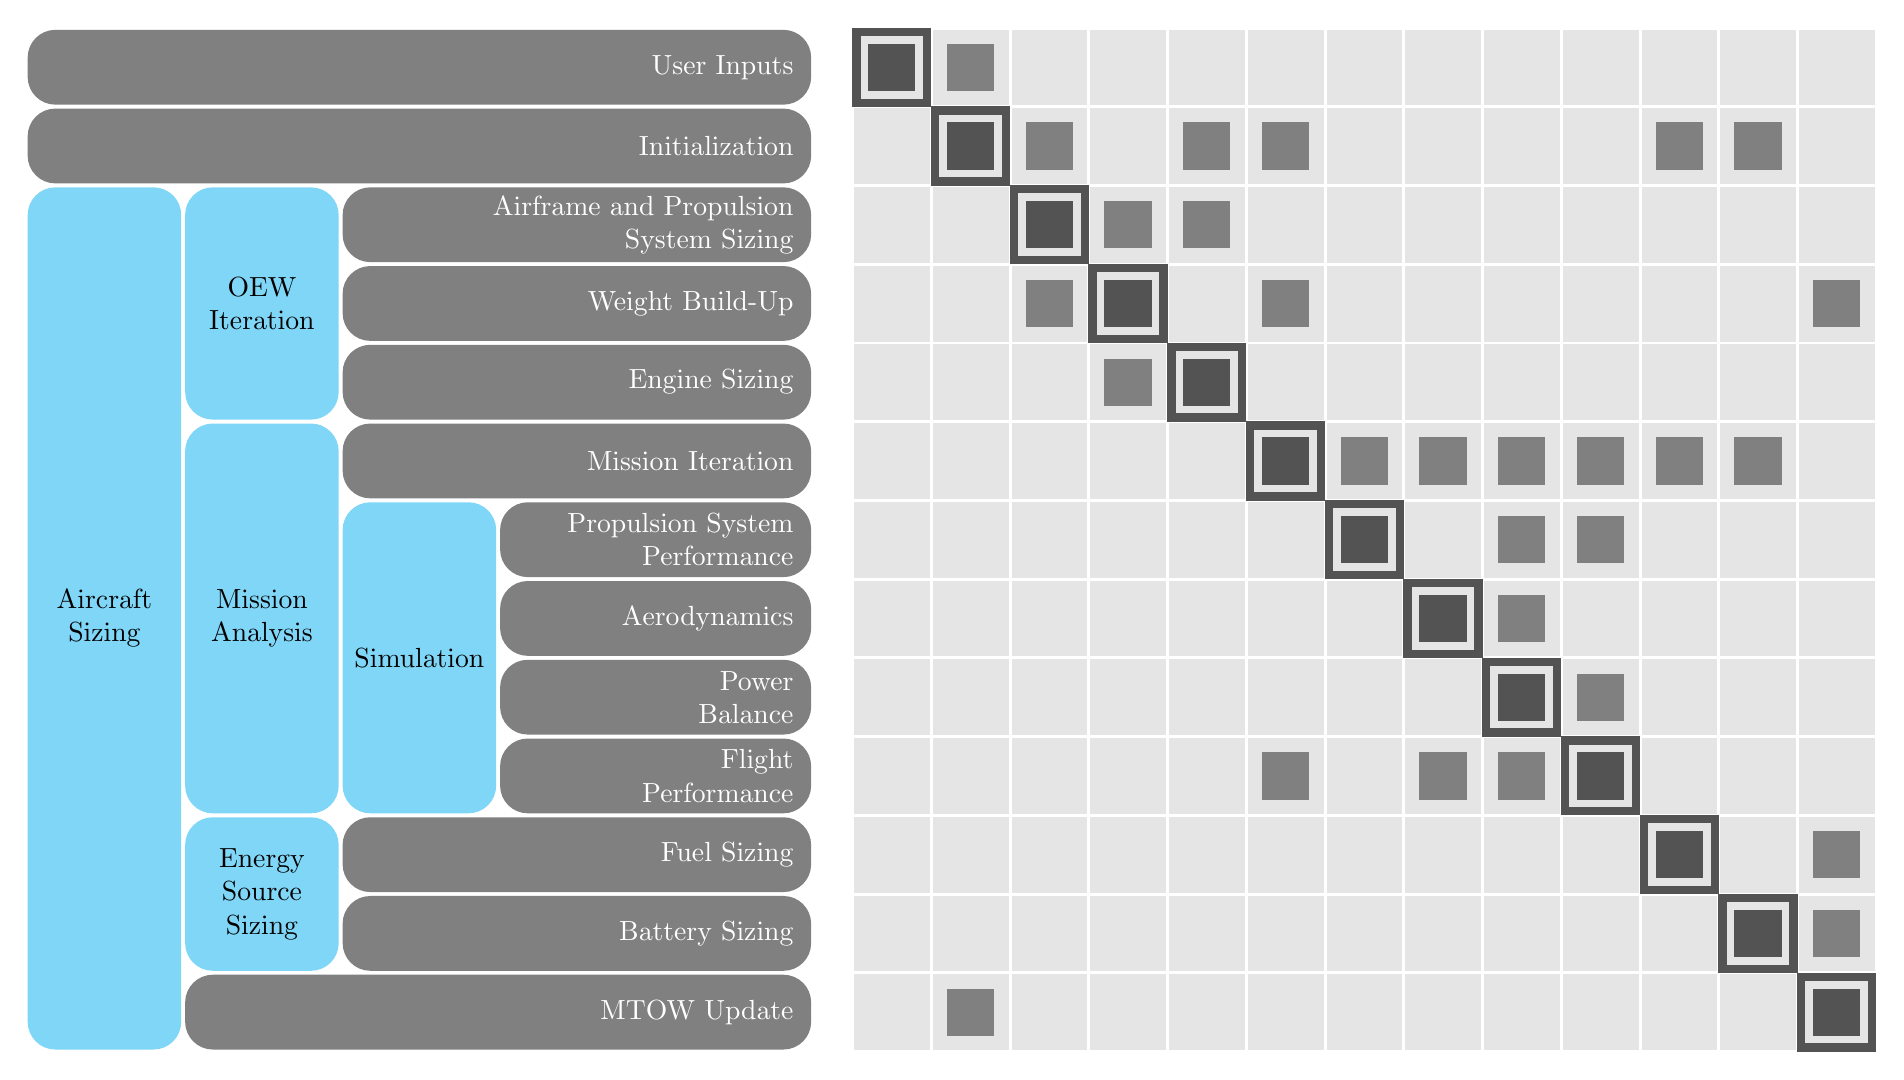
\begin{tikzpicture}[
    on grid,
    every node/.style={
        inner sep=0pt,
        outer sep=0pt,
    },
    outer/.style={
        draw=gray!65!black,rectangle,
        line width=3pt,
        minimum size=.9cm,
    },
    inner/.style={
        fill=#1,rectangle,
        line width=3pt,
        minimum size=.6cm,
    },
    background/.style={
        draw=white,
        line width=.25pt,
        rectangle,
        minimum size=.975cm,
        fill=gray!20,
    },
    leftnodea/.style n args={2}{
        fill=cyan!50,
        align=center,
        % font=\large,
        minimum width=#1 cm-.05cm,
        minimum height=#2 cm-.05cm,
        rounded corners=10pt,
    },
    leftnodeb/.style n args={2}{
        fill=gray,
        align=right,
        text width=#1cm -.5cm,% 
        text=white,
        % font=\large,
        minimum width=#1 cm-.05cm,
        minimum height=#2 cm-.05cm,
        rounded corners=10pt,
    }
]
    \foreach \x in {0,...,12}{
        \foreach \y in {0,...,12}{
            \node[background] at (\x,\y) {};
        }
    }
    \foreach \x [evaluate=\x as \y using 12-\x] in {0,...,12}
    {
        \node[outer] at (\x,\y) {};
        \node[inner=gray!65!black] at (\x,\y) {};
    }
    \foreach \x/\y in {%
        1/12,
        2/11,4/11,5/11,10/11,11/11,
        3/10,4/10,
        2/9,5/9,12/9,
        3/8,
        6/7,7/7,8/7,9/7,10/7,11/7,
        8/6,9/6,
        8/5,
        9/4,
        5/3,7/3,8/3,
        12/2,
        12/1,
        1/0%no comma after
    }{
        \node[inner=gray] at (\x,\y) {};
    }
    \begin{scope}[xshift=-1cm]
    \node[leftnodeb={8}{1}] at (-4,0) {MTOW Update};
    \node[leftnodeb={6}{1}] at (-3,1) {Battery Sizing};
    \node[leftnodeb={6}{1}] at (-3,2) {Fuel Sizing};
    \node[leftnodeb={4}{1}] at (-2,3) {Flight\\Performance};
    \node[leftnodeb={4}{1}] at (-2,4) {Power\\Balance};
    \node[leftnodeb={4}{1}] at (-2,5) {Aerodynamics};
    \node[leftnodeb={4}{1}] at (-2,6) {Propulsion System\\Performance};
    \node[leftnodeb={6}{1}] at (-3,7) {Mission Iteration};
    \node[leftnodeb={6}{1}] at (-3,8) {Engine Sizing};
    \node[leftnodeb={6}{1}] at (-3,9) {Weight Build-Up};
    \node[leftnodeb={6}{1}] at (-3,10) {Airframe and Propulsion\\System Sizing};
    \node[leftnodeb={10}{1}] at (-5,11) {Initialization};
    \node[leftnodeb={10}{1}] at (-5,12) {User Inputs};
    \node[leftnodea={2}{11}] at (-9,5) {Aircraft\\Sizing};
    \node[leftnodea={2}{2}] at (-7,1.5) {Energy\\Source\\Sizing};
    \node[leftnodea={2}{5}] at (-7,5) {Mission\\Analysis};
    \node[leftnodea={2}{3}] at (-7,9) {OEW\\Iteration};
    \node[leftnodea={2}{4}] at (-5,4.5) {Simulation};
    \end{scope}
\end{tikzpicture}

\end{document}